\chapter{Discussion and Conclusion}
\label{discuss} % Always give a unique label

Compare shaft, cannula, sleeve - accuracy, hysteresis.

This is our conclusion)

For future work ..
However, disadvantages would be addition of the cost to already expensive system and possible biocompaitibily and sterilization issues. Also addition of the weight to the arm could alter robot performance, however, since the device will be placed close to center of rotation of the robot arm, it will have minimal affect on the moment of inertia  in comparison to sensors added to the grippers.

Bio-compatibility and coatings

Sterilization techniques

Since 

\begin{figure}[h]
	\begin{center}
		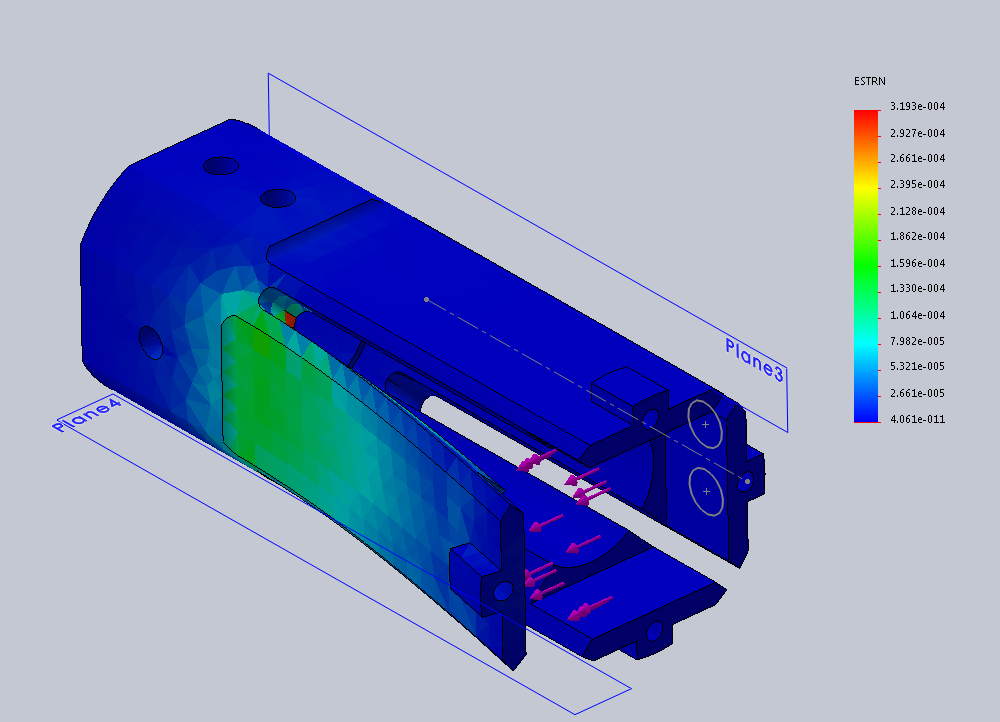
\includegraphics[width=120mm]{fig/methods/NEW_SLEEVE_STRAIN.png}
	\end{center}
	\vspace{-4mm}
	\caption[Setup to measure elasticity modulus]
	{Setup to measure elasticity modulus}
	\label{fig:ElasModSet}
	\vspace{-2mm}
\end{figure}

Z-direction. We tried to measure force in Z-direction, but unfortunately results shown that developed system was not accurate and sensitive enough. To improve system we can suggest to change strain gauges to more sensitive ones. Since we have small room for deformation - around 0.3 mm, we can not afford more deformation by using thinner or longer plates. Therefore, we decided to use motor current readings for z-directional reading of the force.

Increase speed form 588 Hz to something higher by change ADC from SPI 

communication to parallel communication. Right now maximum frequency is 
250ksps, which is 250k/32 = 7.812 KBps.

 Change communication channel bw microcontroller and PC to faster one. Right 
 now we use serial port, with max speed 7.1 KBps 
 
Change microcontroller to the faster one. 

We can use QTC-pills in future, promising approach, higher sensitivity 